%!TEX root = ../../csuthesis_main.tex
\chapter{图像布局}
\label{sec.figure}
\section{单图布局}

TeX (/tɛx, tɛk/, see below), stylized within the system as TEX, is a typesetting system (or a "formatting system") which was designed and mostly written by Donald Knuth[1] and released in 1978. TeX is a popular means of typesetting complex mathematical formulae; it has been noted as one of the most sophisticated digital typographical systems.


\textbf{单图布局如图\ref{F.csu_single}所示。}

\begin{figure}[hbt]
\centering
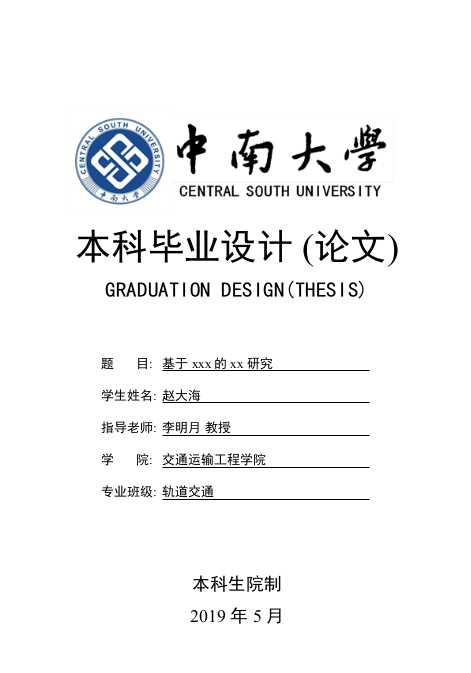
\includegraphics[width=0.5\textwidth]{csu.png}
\caption{单图布局示例}
\label{F.csu_single}
\end{figure}

\section{横排布局}

\textbf{横排布局如图\ref{F.csu_row}所示。}

\begin{figure}[!htb]
    \centering
    \begin{subfigure}[t]{0.24\linewidth}
        \begin{minipage}[b]{1\linewidth}
        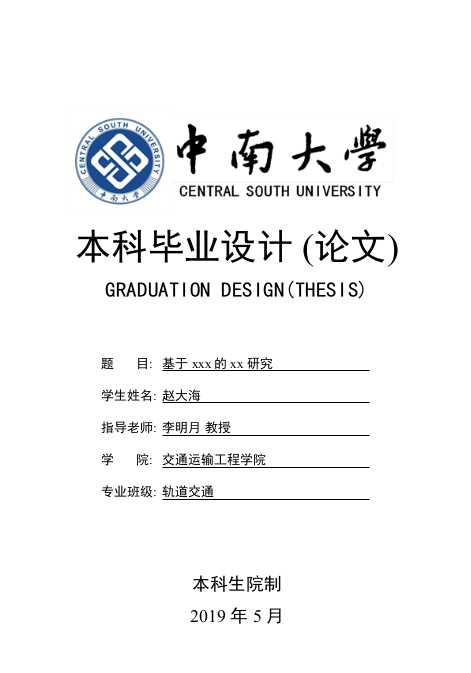
\includegraphics[width=1\linewidth]{csu.png}
        \caption{test}
        \end{minipage}
    \end{subfigure}
    \begin{subfigure}[t]{0.24\linewidth}
        \begin{minipage}[b]{1\linewidth}
        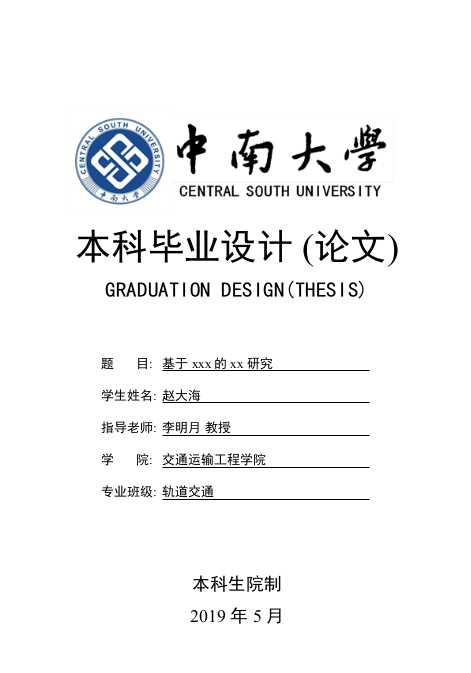
\includegraphics[width=1\linewidth]{csu.png}
        \caption{test}
        \end{minipage}
    \end{subfigure}
    \begin{subfigure}[t]{0.24\linewidth}
        \begin{minipage}[b]{1\linewidth}
        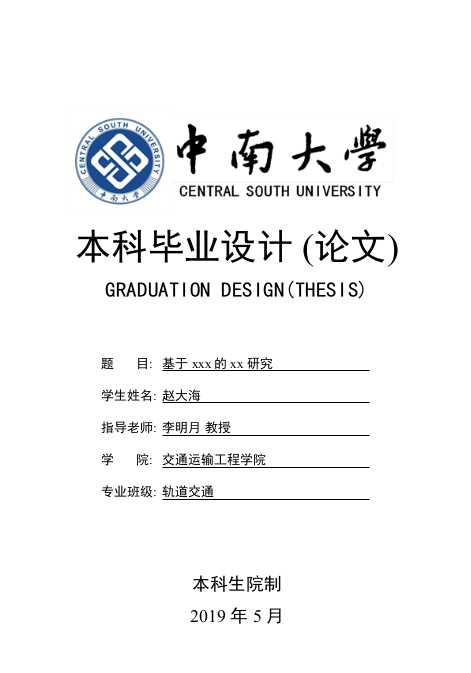
\includegraphics[width=1\linewidth]{csu.png}
        \caption{test}
        \end{minipage}
    \end{subfigure}
    \begin{subfigure}[t]{0.24\linewidth}
        \begin{minipage}[b]{1\linewidth}
        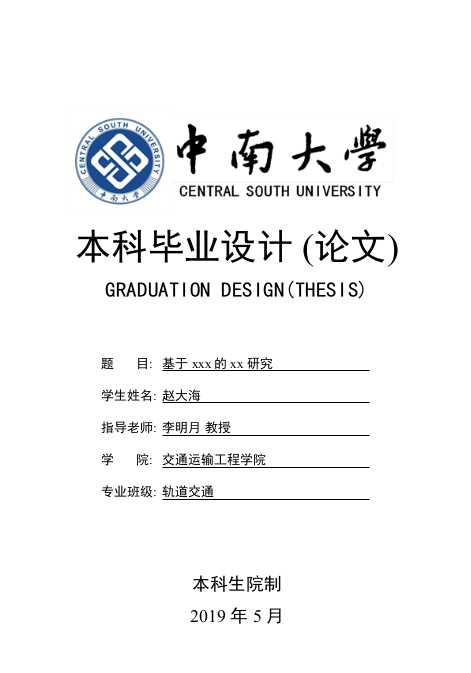
\includegraphics[width=1\linewidth]{csu.png}
        \caption{test}
        \end{minipage}
    \end{subfigure}
    \caption{横排布局示例}
    \label{F.csu_row}
\end{figure}

TeX (/tɛx, tɛk/, see below), stylized within the system as TEX, is a typesetting system (or a "formatting system") which was designed and mostly written by Donald Knuth[1] and released in 1978. TeX is a popular means of typesetting complex mathematical formulae; it has been noted as one of the most sophisticated digital typographical systems.


\section{竖排布局}
\textbf{竖排布局如图\ref{F.csu_col}所示。}

\begin{figure}[!htb]
    \centering
    \begin{subfigure}[t]{0.15\linewidth}
        \captionsetup{justification=centering} %ugly hacks
        \begin{minipage}[b]{1\linewidth}
        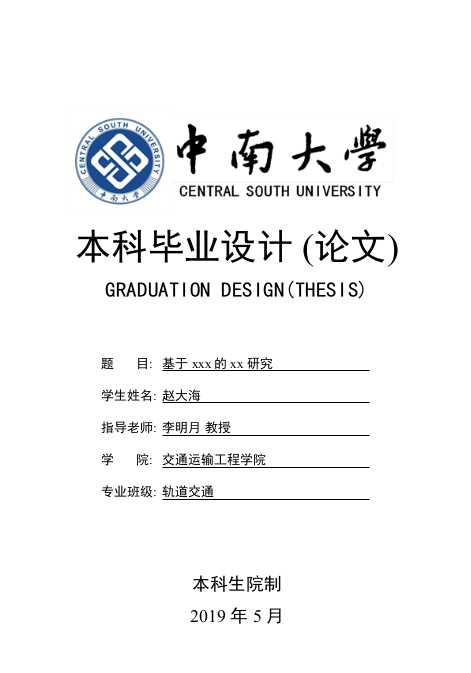
\includegraphics[width=1\linewidth]{csu.png}
        \caption{test}
        \end{minipage}
    \end{subfigure}\\
    \begin{subfigure}[t]{0.15\linewidth}
        \captionsetup{justification=centering} %ugly hacks
        \begin{minipage}[b]{1\linewidth}
        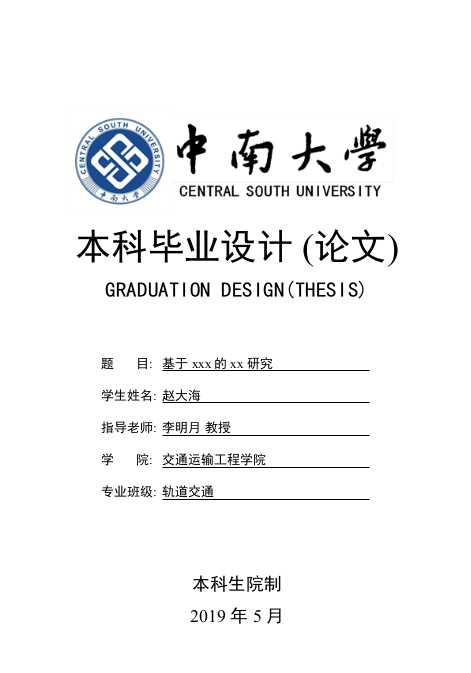
\includegraphics[width=1\linewidth]{csu.png}
        \caption{test}
        \end{minipage}
    \end{subfigure}
    \caption{竖排布局示例}
    \label{F.csu_col}
\end{figure}

TeX (/tɛx, tɛk/, see below), stylized within the system as TEX, is a typesetting system (or a "formatting system") which was designed and mostly written by Donald Knuth[1] and released in 1978. TeX is a popular means of typesetting complex mathematical formulae; it has been noted as one of the most sophisticated digital typographical systems.


\section{竖排多图横排布局}

\begin{figure}[!htb]
    \centering
    \begin{subfigure}[t]{0.13\linewidth}
        \captionsetup{justification=centering} 
        \begin{minipage}[b]{1\linewidth}
        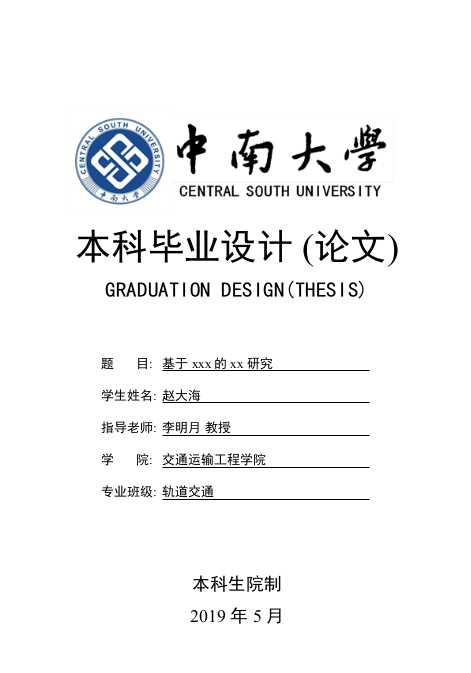
\includegraphics[width=1\linewidth]{csu.png} \vspace{-1ex} \vfill
        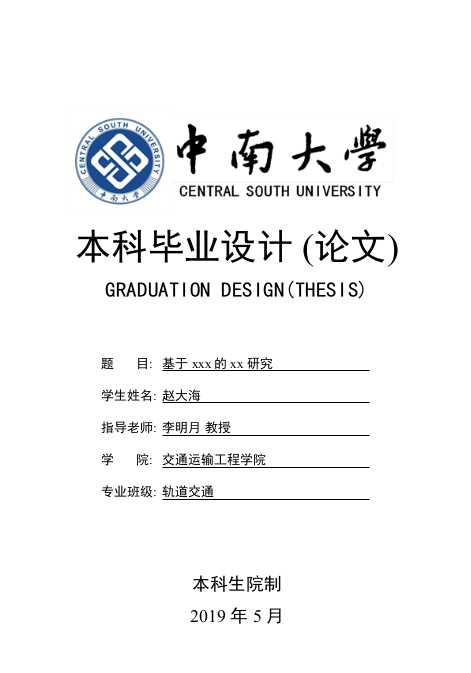
\includegraphics[width=1\linewidth]{csu.png}
        \caption{aaa}
        \end{minipage}
    \end{subfigure}
    \begin{subfigure}[t]{0.13\linewidth}
        \captionsetup{justification=centering} 
        \begin{minipage}[b]{1\linewidth}
        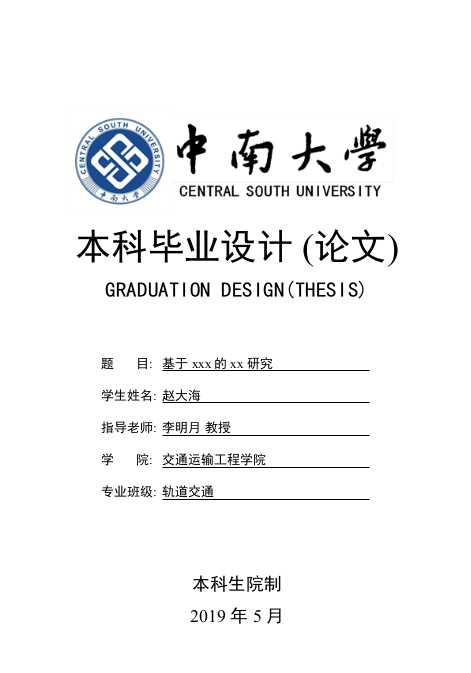
\includegraphics[width=1\linewidth]{csu.png} \vspace{-1ex} \vfill
        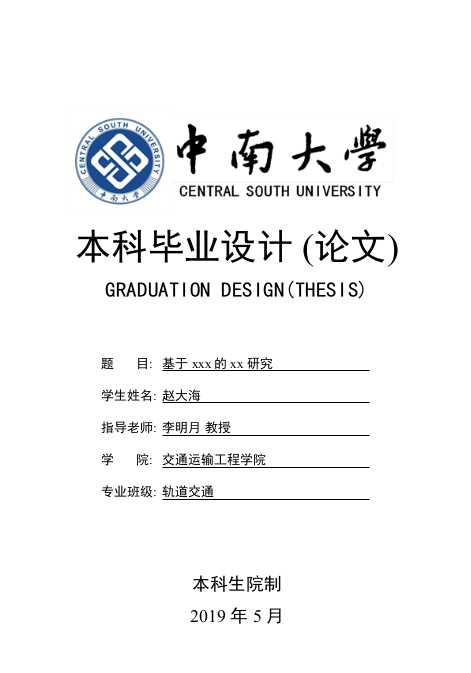
\includegraphics[width=1\linewidth]{csu.png}
        \caption{bbb}
        \end{minipage}
    \end{subfigure}
    \caption{竖排多图横排布局}
    \label{F.csu_col_row}
\end{figure}

\textbf{竖排多图横排布局如图\ref{F.csu_col_row}所示。注意看(a)、(b)编号与图关系。}


\section{横排多图竖排布局}

中南大学由原湖南医科大学、长沙铁道学院与中南工业大学于2000年4月合并组建而成。原中南工业大学的前身为创建于1952年的中南矿冶学院,原长沙铁道学院的前身为创建于1953年的中南土木建筑学院,两校的主体学科最早溯源于1903年创办的湖南高等实业学堂的矿科和路科。原湖南医科大学的前身为1914年创建的湘雅医学专门学校,是我国创办最早的西医高等学校之一。中南大学秉承百年办学积淀,顺应中国高等教育体制改革大势,弘扬以“知行合一、经世致用”为核心的大学精神,力行“向善、求真、唯美、有容”的校风,坚持自身办学特色,服务国家和社会重大需求,团结奋进,改革创新,追求卓越,综合实力和整体水平大幅提升。

\begin{figure}[!htb]
    \centering
    \begin{subfigure}[t]{0.3\linewidth}
        \captionsetup{justification=centering} 
        \begin{minipage}[b]{1\linewidth}
        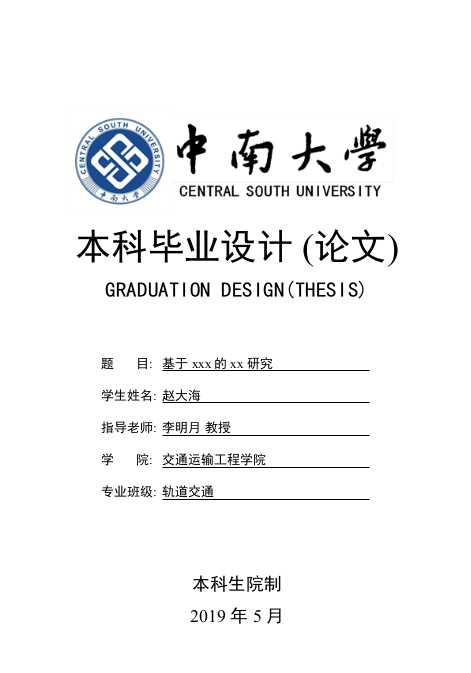
\includegraphics[width=0.45\linewidth]{csu.png}
        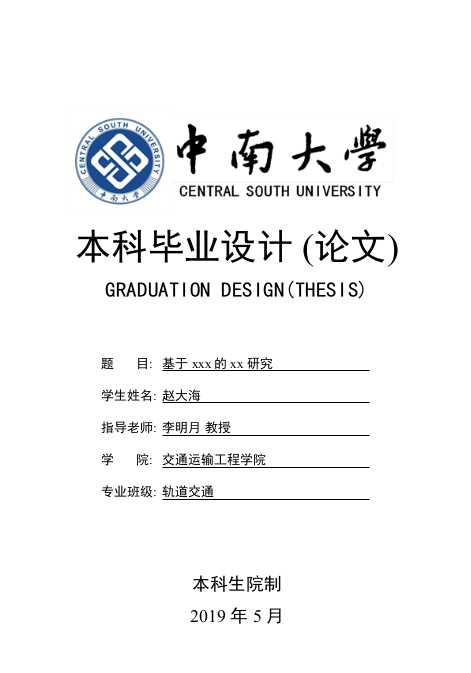
\includegraphics[width=0.45\linewidth]{csu.png}
        \caption{}
        \end{minipage}
    \end{subfigure}\\
    \begin{subfigure}[t]{0.3\linewidth}
        \captionsetup{justification=centering} 
        \begin{minipage}[b]{1\linewidth}
        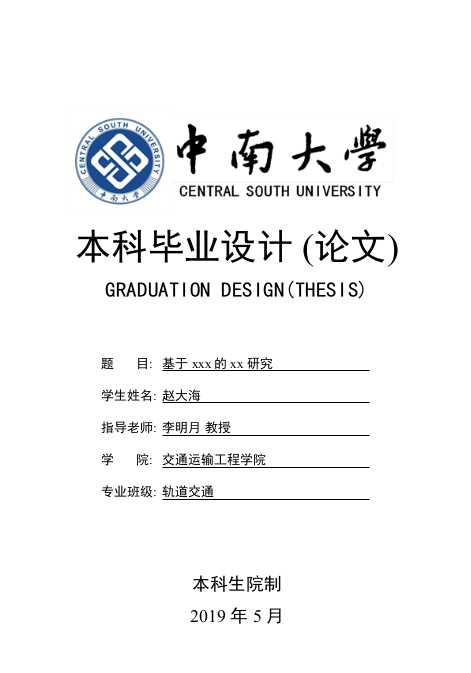
\includegraphics[width=0.45\linewidth]{csu.png}
        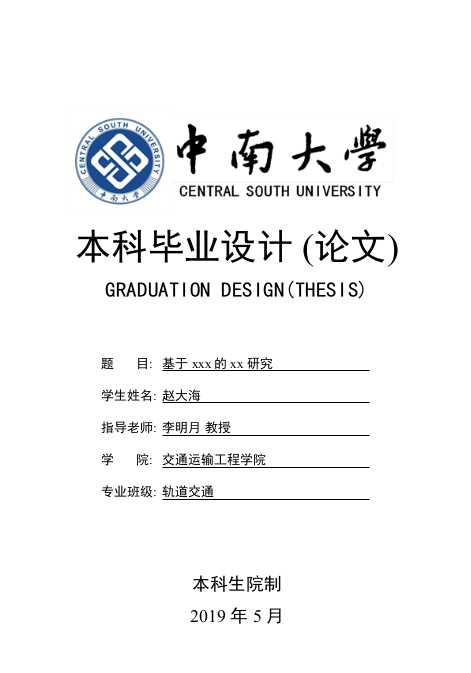
\includegraphics[width=0.45\linewidth]{csu.png}
        \caption{}
        \end{minipage}
    \end{subfigure}
    \caption{横排多图竖排布局}
    \label{F.csu_row_col}
\end{figure}

\textbf{横排多图竖排布局如图\ref{F.csu_row_col}所示。注意看(a)、(b)编号与图关系。}

\section{本章小结}
本章示例图片布局。

